%% !TeX program = lualatex

%\listfiles	
% **************************
% STOP - Bitte zuerst lesen, bevor Sie weitermachen
%
% Einige Dinge müssen Sie an Ihre Bedürfnisse (und die Vorgaben Ihres
% Betreuers anpassen. Editieren Sie dazu die Datei docinfo.tex).
%
% 1. Sprache
% Das Template unterstützt Deutsch und Englisch, Standard ist Deutsch.
% Wenn Sie Englisch verwenden wollen, ändern Sie bitte direkt am Anfang
% dieser Datei den Eintrag
%    \newcommand{\hsmasprache}{de}
% auf
%    \newcommand{\hsmasprache}{en}
%
% 2. Form der Abgabe
% Das Template unterstützt sowohl eine digitale Abgabe, als auch eine Abgabe
% auf Papier. Bei einer Papierabgabe wird ein doppelseitiger Druck vorbereitet
% und der Titel wird so platziert, dass er in das Fenster des offiziellen
% Umschlages der Technischen Hochschule passt.
% Bei einer digitalen Abgabe (als PDF) wird der Titel zentriert und als
% Format wird einseitig gewählt. Außerdem wird die Datei unterschrift.png
% auf dem Blatt mit der Erklärung zur Eigenständigkeit eingebunden.
%
% 3. Zitierstil
% Abhängig von dem gewünschten Zitierstil passen Sie bitte in
% hma.cls die Einstellungen bei \RequirePackage[backend=biber...
% an. Wie ist dort genau erklärt.
% Achtung: Wenn Sie als Zitierstil Fußnoten wählen bzw. generell
% -------  mit Fußnoten arbeiten, dann beachten Sie bitte, dass
%          Fußnoten in Bildunterschriften und Tabellenüberschriften
%          nicht funktionieren.
%          Siehe hierzu https://texfaq.org/FAQ-ftncapt
%          und https://texfaq.org/FAQ-footintab
%          Sinnvollerweise verzichten Sie auf Fußnoten an diesen
%          Stellen und fügen Quellen einfach per \parancite ein.
%
% 4. Doppelseitiger oder einseitiger Druck
% Das Template bestimmt, ob einseitig oder doppelseitig gedruckt wird
% anhand der Abgabeform (papier / digital). Wollen sie dies übersteuern,
% müssen Sie in der Datei preambel.tex folgende Zeile
% \KOMAoptions{twoside=true} für doppelsetigen Druck
% \KOMAoptions{twoside=false} für einsetigen Druck
% direkt vor \usepackage{xcolor} einsetzen. Prinzipiell sollten Sie aber
% das vorgeschlagene Format einfach so lassen.
%
% 5. Unnötige Teile entfernen
% Entfernen Sie die Teile, die Sie nicht brauchen, z.B. Anhänge
%
% 6. Silbentrennung
% LaTeX führt eine automatische Silbentrennung durch. Allerdings
% werden Wörter, die bereits einen Bindestrich enthalten nicht
% getrennt, z.B. Datenschutz-Grundverordnung. Wenn Sie Ihren Text auf
% Deutsch schreiben, können Sie dann alternativ "= für den Bindestrich
% im Wort verwenden, z.B. Datenschutz"=Grundverordnung, damit LaTeX
% weiterhin richtig trennt.
% Ist die Silbentrennung aus einem anderen Grund nicht erfolgt, sodass
% das Wort über den rechten Rand hinaussteht oder wenn Sie eine weitere
% Trennstelle wollen, können Sie LaTeX helfen, indem Sie weitere
% Trennstellen angeben. Dies geschieht durch "- als Zeichen, z.B.
% Staats"-vertrag.
%
% 7. Nummerierung der Fußnoten
% LaTeX beginnt die Nummerierung der Fußnoten in jedem Kapitel wieder
% bei 1. In diesem Template wird die fortlaufende Nummerierung der Fußnoten 
% über die gesamte Arbeit umgesetzt.  
%
% 8. Unterschrift
% Bei einer Abgabe auf Papier unterschreiben Sie die Arbeit eigenhändig.
% Geben Sie allerdings digital ab, sollten Sie die Datei unterschrift.png in dem 
% Ordner /bilder durch einen Scan Ihrer eigenen Unteschrift ersetzen - andernfalls
% unterschreiben Sie als Max Mustermann ;-)
% *******************************************************************


% Dokumenteneinstellungen und Infos importieren
% -------------------------------------------------------
% Informationen und Einstellungen für Ihre Abschlussarbeit
%

% Sprache für das Dokument festlegen
\newcommand{\hsmasprache}{de} %de für Deutsch oder en für Englisch


% Abgabeform festlegen
% Bei einer digitalen Abgabe, wird das Dokument einseitig erzeugt und der Titel wird
% zentriert.
\newcommand{\hsmaabgabe}{digital} % Abgabe erfolgt für Fakultät I digital. Optionen hier sind für anderen Fakultäten: "papier" oder "digital".


% Flags für Veröffentlichung, Sperrvermerk
\newcommand{\hsmapublizieren}{opensource}   
% Wird einer Veröffentlichung zugestimmt?
% Optionen: 
% opensource = Druck der CC Lizenz mit By SA (Standard)
% hs = Veröffentlichung an der Technischen Hochschule und auf Hochschulservern
% stud = kein opensource und keine veröffentlichung auf den Hochschulservern
% vertraulich = Arbeit darf nicht veröffentlicht werden und erhält einen Sperrvermerk (Nur nach Absprache mit Betreuer setzen!)


\newcommand{\genderhinweis}{gender}     % Soll der Gender-Hinweis angezeigt werden? ja=gender, nein = nogender; Genderhinweis wird nur in deutscher Sprache angezeigt!


\newcommand{\hsmaquellcode}{sourcecode} % Verwenden Sie Quellcode in Ihrer Arbeit? ja=sourcecode, nein= nosourcecode

\newcommand{\hsmasymbole}{symbole} % Verwenden Sie viele Symbole in Ihrer Arbeit, welche in einem Symbolverzeichnis aufgeführt werden sollen? ja=symbole, nein= nosymbole


\newcommand{\hsmaglossar}{glossar} % Verwenden Sie Begriffserklärungen nicht Abkürzungen in Ihrer Arbeit? ja=glossar, nein= noglossar

\newcommand{\hsmatc}{tc} % Verwenden der Änderungsmarkierung. Änderungsmarkierung aktiv und eine Liste der Änderungen wird angezeigt = tc, Keine Änderungsmarkierung und keine Ausgabe der Änderungen = notc




% Titel der Arbeit auf Deutsch
\newcommand{\hsmatitelde}{Eindeutige Produktzuordnung zur Schwachstellenanalyse: Modellierung von Produkten zur Abbildung mit heterogenenen Schwachstellendatenbanken}

% Titel der Arbeit auf Englisch
\newcommand{\hsmatitelen}{AUTO-TRANSLATED: Unambiguous Product Mapping for Vulnerability Analysis: Modeling of Products for Integration with Heterogeneous Vulnerability Databases}

% Weitere Informationen zur Arbeit
\newcommand{\hsmaort}{Mannheim}        % Ort
\newcommand{\hsmaautorvname}{Yan}      % Vorname(n)
\newcommand{\hsmaautornname}{Wittmann} % Nachname(n)
\newcommand{\hsmaabgabedatum}{2025-07-21} % Datum der Abgabe in dem Format JJJJ-MM-TT

\newcommand{\hsmafirma}{\{metæffekt\} GmbH} % Firma bei der die Arbeit durchgeführt wurde
\newcommand{\hsmabetreuer}{Prof. Thomas Smits, Technische Hochschule Mannheim} % Betreuer an der Hochschule
\newcommand{\hsmazweitkorrektor}{Karsten Klein, \{metæffekt\} GmbH}   % Betreuer im Unternehmen oder Zweitkorrektor

\newcommand{\hsmafakultaet}{I}    % I für Informatik oder E, S, B, D, M, N, W, V
\newcommand{\hsmastudiengang}{IB} % IB IMB UIB CSB IM MTB (weitere siehe titleblatt.tex)


% Preambel importieren
% Dokumententyp, benutzte Pakete und deren Einstellungen
\documentclass[	\hsmasprache,%
				\hsmaabgabe,%
				\hsmapublizieren,%
				\genderhinweis,
				\hsmaquellcode,
				\hsmasymbole,
				\hsmaglossar,
				\hsmatc]{HMA}

% Wo sind die Bilder?
\graphicspath{{bilder/}}


% Wo liegt Sourcecode?
\newcommand{\srcloc}{src/}


% Checklisten mit zwei Ebenen
\newlist{checklist}{itemize}{2}
\setlist[checklist]{label=$\square$}



% Befehl zum Erstellen eigener Makros. In diesem Fall ist es ein Makro für das Einbinden von Bildern. Das label (für \ref) ist dann der Name der Bilddatei
\newcommand{\bild}[3]{
	\begin{figure}[ht]
		\centering
		\includegraphics[width=#2]{#1}
		\caption{#3}
		\label{#1}
\end{figure}}




							


\newcommand{\snowcard}[9]{
	\begin{table}[ht!]
		\caption{\hsmasnowcardanforderung\ #1 -- #4}\label{#1}
		\renewcommand{\arraystretch}{1.2}
		\centering
		\sffamily
		\begin{footnotesize}

			\begin{tabularx}{\linewidth}{sssssl}
				\toprule
				\textbf{\hsmasnowcardno} & #1 & \textbf{\hsmasnowcardart} & #2 & \textbf{\hsmasnowcardprio} & #3 \\
				\midrule
				\multicolumn{2}{l}{\textbf{\hsmasnowcardtitel}} & \multicolumn{4}{l}{\parbox[t]{11.8cm}{#4}} \\
				\ifx&#5&%
				\else
				\multicolumn{2}{l}{\textbf{\hsmasnowcardherkunft}} & \multicolumn{4}{l}{\parbox[t]{11.8cm}{#5}} \\
				\fi
				\ifx&#6&%
				\else
				\multicolumn{2}{l}{\textbf{\hsmasnowcardkonflikt}} & \multicolumn{4}{l}{\parbox[t]{11.8cm}{#6}} \\
				\fi
				\addlinespace
				\multicolumn{6}{l}{\textbf{\hsmasnowcardbeschreibung}} \\
				\multicolumn{6}{l}{\parbox[t]{13.5cm}{#7\strut}} \\
				\ifx&#8&%
				\else
				\addlinespace
				\multicolumn{6}{l}{\textbf{\hsmasnowcardfitkriterium}} \\
				\multicolumn{6}{l}{\parbox[t]{13.5cm}{#8\strut}} \\
				\fi
				\ifx&#9&%

				\else
				\addlinespace
				\multicolumn{6}{l}{\textbf{\hsmasnowcardmaterial}} \\
				\multicolumn{6}{l}{\parbox[t]{13.5cm}{#9\strut}} \\
				\fi
				\bottomrule
			\end{tabularx}
		\end{footnotesize}
	\end{table}
}



% Quality Attribute Scenario
\newcommand{\qas}[9]{
	\begin{table}[ht!]
		\caption{\hsmaqasanforderung\ #1 -- #3}\label{#1}
		\renewcommand{\arraystretch}{1.2}
		\centering
		\sffamily
		\begin{footnotesize}

			\begin{tabularx}{\linewidth}{sssssl}
				\toprule
				\textbf{\hsmaqasno} & #1 & \textbf{\hsmaqasart} & QAS & \textbf{\hsmaqasprio} & #2 \\
				\midrule
				\multicolumn{2}{l}{\textbf{\hsmaqastitel}} & \multicolumn{4}{l}{\parbox[t]{11.8cm}{#3}} \\
				\multicolumn{2}{l}{\textbf{\hsmaqasquelle}} & \multicolumn{4}{l}{\parbox[t]{11.8cm}{#4}} \\
				\multicolumn{2}{l}{\textbf{\hsmaqasstimulus}} & \multicolumn{4}{l}{\parbox[t]{11.8cm}{#5}} \\
				\multicolumn{2}{l}{\textbf{\hsmaqasartefakt}} & \multicolumn{4}{l}{\parbox[t]{11.8cm}{#6}} \\
				\addlinespace
				\multicolumn{6}{l}{\textbf{\hsmaqasumgebung}} \\
				\multicolumn{6}{l}{\parbox[t]{13.5cm}{#7\strut}} \\
				\addlinespace
				\multicolumn{6}{l}{\textbf{\hsmaqasantwort}} \\
				\multicolumn{6}{l}{\parbox[t]{13.5cm}{#8\strut}} \\
				\addlinespace
				\multicolumn{6}{l}{\textbf{\hsmaqasmass}} \\
				\multicolumn{6}{l}{\parbox[t]{13.5cm}{#9\strut}} \\
				\bottomrule
			\end{tabularx}
		\end{footnotesize}
	\end{table}
}




%Abstrakt Ihrer Abschlussarbeit
% -------------------------------------------------------
% Abstrakt / Abstract
% Achtung: Wenn Sie im Abstrakt Anführungszeichen verwenden wollen, dann benutzen Sie
%          nicht "` und "', sondern \enquote{}. "` und "' werden nicht richtig
%          erkannt.

% Kurze (maximal halbseitige) Beschreibung, worum es in der Arbeit geht auf Deutsch
\newcommand{\hsmaabstractde}{
    Um Softwareartefakte verschiedenen Produktrepräsentationen wie CPE, PURL oder Produktkennungen von Microsoft zuordnen zu können, wurde in dieser Arbeit ein neues System für die Modellierung von Beziehungen zwischen Produkten für das Schwachstellen\-management-System der \metaeffektsp GmbH entwickelt.
    Ausgangspunkt ist eine Analyse der Schwächen des bisherigen YAML-basierten Formats, darunter die Übergeneralisierung von Regeln zur Auswahl von Artefakten, uneinheitliche Typangaben und eingeschränkt nachvollziehbare Entscheidungen.
    Als Lösung wurde ein graphenbasiertes Modell entworfen, in dem Produkte und ihre verschiedenen Darstellungen als Knoten erfasst und ihre Beziehungen durch Kanten beschrieben werden.
    Dieses Modell wurde in Java zur Demonstration der Funktionsfähigkeit umgesetzt und nutzt SQLite zur Speicherung der Daten.
    Durch eine Analyse der möglichen Datenquellen werden im neuen System typische Merkmale der Daten genutzt, um typspezifische Attribute für genauere und bewusstere Zuordnungen explizit bereitzustellen.
    Manuelle Anpassungen bleiben weiterhin über ein manuelles Modifikationsformat möglich.
    Zudem wird die automatische Generierung von Inahlten aus öffentlichen Datenanteilen und innere Konsistenzprüfung behandelt.
}

% Kurze (maximal halbseitige) Beschreibung, worum es in der Arbeit geht auf Englisch
\newcommand{\hsmaabstracten}{
    In order to reliably assign software artefacts to various product representations such as CPEs, PURLs, or Microsoft product identifiers, this thesis presents the development of a new system for modeling relationships between products for the vulnerability management system of \metaeffektsp GmbH.
    The work begins with an analysis of the limitations of the existing YAML-based correlation solution, which include overly broad selection rules, inconsistent type matching, and limited traceability of decision logic.
    As a solution, a graph-based model was designed, in which products and their representations are expressed as nodes, and their relationships are described through typed edges.
    This model was implemented in Java to demonstrate its feasibility and uses SQLite for data storage.
    Based on an analysis of common input sources, the new system identifies characteristic patterns to extract type-specific attributes, enabling more accurate and deliberate correlations.
    Manual adjustments remain possible by applying a dedicated modification format.
    The system also addresses the automated generation of graph contents from public data sources and ensures internal consistency through validation mechanisms
}



% Literatur-Datenbank
\addbibresource{literatur.bib}   % BibLaTeX-Datei mit Literaturquellen einbinden


% Anfang des Dokuments
\begin{document}	


%Laden der Dateien mit Abkürzungen, Begriffserklärungen (Glossar), Symbole
\newacronym{oss}{OSS}{Open Source Software}
\newacronym{cra}{CRA}{Cyber Resilliance Act}
\newacronym{cve}{CVE}{Common Vulnerabilities and Exposures}
\newacronym{cpe}{CPE}{Common Product Enumeration}
\newacronym{osv}{OSV}{Open Source Vulnerabilities}
\newacronym{msrc}{MSRC}{Microsoft Security Responce Center}
\newacronym{nist}{NIST}{National Institute of Standards and Technology}
\newacronym{vms}{VMS}{Vulnerability Management System}
\newacronym{vdb}{VDB}{Vulnerability Database}
\newacronym{nvd}{NVD}{National Vulnerability Database}
\newacronym{purl}{PURL}{Package URL}
\newacronym{cwe}{CWE}{Common Weakness Enumeration}
\newacronym{ciavuln}{CIA}{Confidentiality, Integrity, Availability}
\newacronym{api}{API}{Application Programming Interface}
\newacronym{cisa}{CISA}{Cybersecurity and Infrastructure Security Agency}
\newacronym[
  plural=CNAs,
  firstplural=CVE Numbering Authorities (CNAs)
]{cna}{CNA}{CVE Numbering Authority}
\newacronym{sbom}{SBOM}{Software Bill of Materials}
\newacronym{spdx}{SPDX}{System Package Data Exchange}
\newacronym{swid}{SWID}{Software Identification Tags}
\newacronym{cmu}{CMU}{Carnegie Mellon University}
\newacronym{scap}{SCAP}{Security Content Automation Protocol}
\newacronym{wfn}{WFN}{Well-Formed CPE Name}
\newacronym{yaml}{YAML}{Yet Another Markup Language}
\newacronym{csv}{CSV}{Comma Separated Value}
\newacronym{ide}{IDE}{Integrated Development Environment}
\newacronym{eol}{EOL}{End of Life (endoflife.date)}
\newacronym{bsi}{BSI}{Bundesamts für Sicherheit in der Informationstechnik}
\newacronym{ai-rnn}{RNN}{rekurrentes neuronales Netzwerk}

% Glossareinträge
\newglossaryentry{glos:amplification}{name={Amplification}, description={describes the disproportionate increase of a response packet compart to the initial request packet.}}

% Verzeichnis von Symbolen und Einheiten
\newglossaryentry{symb:Pi}{name=\ensuremath{\pi},
	description={Geometrical value},
	unit={},
	type=symbolslist}

\newglossaryentry{symb:energyconsump}{name=\ensuremath{P},
	description={Energy consumption},
	unit={\si{kW}},
	type=symbolslist}
	
	
\pagestyle{headings}
\tableofcontents


\mainmatter

%% Ihre Inhaltsdateien werden an dieser Stelle in das Dokument eingefügt
\chapter{Einleitung}\label{ch:einleitung}


\section{Hintergrund und Motivation}\label{sec:hintergrund-motivation}

Moderne Software wird zunehmend aus einer Vielzahl kleinerer Bestandteile zusammengesetzt, was die Art und Weise, wie Software entwickelt, verteilt und betrieben wird, grundlegend verändert hat.
Ein großer Anteil dieser Komponenten basiert auf \acrfull{oss} und dient damit als Grundlage digitaler Infrastrukturen in nahezu allen Branchen:
Laut dem Open Source Monitor des Bitkom e.V.\ setzen 69\% der deutschen Unternehmen \acrshort{oss} in ihren Lösungen ein\ \autocite{OpenSourceMonitorWintergerst}.

Mit der wachsenden Abhängigkeit von \acrshort{oss} steigt jedoch auch die Verantwortung für deren sichere und nachvollziehbare Verwendung.
In dem bereits verabschiedeten \acrfull{cra} der Europäischen Union geht es um die Cybersicherheit von Produkten mit digitalen Elementen und berücksichtigt dabei auch \acrshort{oss}-Komponenten.
Ab dem 11.\ Juni 2026 sind Unternehmen verpflichtet, bekannte Schwachstellen in ihrer Software-Lösung und den verwendeten Komponenten zu identifizieren und Sicherheitsvorfälle zu dokumentieren.
Spätestens ab dem 11.\ Dezember 2027 sind alle Vorgaben des \acrshort{cra} verbindlich.
Eine aktiv ausgenutzte Schwachstelle ist nach dem \acrshort{cra} ein meldepflichtiger Sicherheitsvorfall und muss innerhalb von 72 Stunden an die zuständigen Behörden gemeldet werden\ \autocite{eu2024cra}.

Eine der am weitesten verbreiteten Quellen für Schwachstelleninformationen ist das \acrfullr{cve}-System, das als Bestandteil der \acrfull{nvd} des \acrfull{nist}\footnote{\url{https://nvd.nist.gov/vuln}} mit derzeit fast 300.000 Einträgen die umfangreichste öffentlich zugängliche Schwachstellendatenbank darstellt\ \autocite{nvd12mai2025dashboard}.
Diese große Anzahl an erfassten Schwachstellen und der kontinuierliche Zuwachs machen es in Kombination mit den kurzen Meldefristen des \acrshort{cra} unmöglich, den Prozess der Schwachstellensuche rein manuell abzubilden.
Für 65\% der Unternehmen ist eine manuelle Überwachung dieser Datenmengen durch den zeitlichen Aufwand und das Risiko eines menschlichen Fehlers unmöglich\ \autocite{OpenSourceMonitorWintergerst}, weshalb sie automatisierte \acrfull{vms} einsetzen.

Moderne und automatisierte \acrshort{vms} verarbeiten die erfassten Softwareinventare typischerweise in mehreren Schritten, um den firmeneigenen Softwarekatalog mit relevanten Schwachstelleninformationen aus verknüpften \acrfullpl{vdb} abzugleichen:
die Identifikation der eingesetzten Komponenten, die Erkennung potenzieller Schwachstellen, eine regelbasierte Bewertung der Ergebnisse und die Erzeugung von Ergebnisberichten\ \autocite{Idrissi_Sebai_Faroukhi_Mahouachi_2024}.

Die Zuordnung der eigenen Komponenten zu den Produktbezeichnern der jeweils abzugleichenden \acrshort{vdb} ist als erster Schritt bereits einer der herausforderndsten.
Die \acrshort{nvd} etwa stellt mit dem \acrfull{cpe}-System ein Schema zur Verfügung, um Softwareprodukte zu identifizieren und zu \acrshort{cve} zuzuordnen\ \autocite{Cheikes_Waltermire_Scarfone_2011}.
In der Praxis ist die korrekte Abbildung der eingesetzen Komponenten auf \acrshort{cpe}-Einträge jedoch mit Schwierigkeiten verbunden:
uneinheitliche Benennungen, Doppelungen, Rechtschreibfehler und mehr führen zu Fehlidentifikationen und unvollständigen Ergebnissen im darauf folgenden Schwachstellen-Scan\ \autocite{Sanguino_Uetz_2017}.
Dies macht es unmöglich, sich ausschließlich auf die Ergebnisse dieser automatischen Scans zu verlassen und erfordert eine manuelle Kontrolle der Ergebnisse, insbesondere der erschlossenen Komponenten-Abbildungen\ \autocite{Sanguino_Uetz_2017}.

Das Problem beschränkt sich jedoch nicht auf die \acrshort{nvd} mit ihren \acrshort{cpe}, auch Produktbezeichner aus anderen Quellen wie die \acrfull{osv}-Datenbank\footnote{\url{https://osv.dev}}, den \acrfull{msrc} Update Guides\footnote{\url{https://msrc.microsoft.com/update-guide}}, endoflife.date\footnote{\url{https://endoflife.date}} und weitere lassen sich nicht ohne weiteres gegenseitig zuordnen.

Die \metaeffekt\ entwickelt seit mehreren Jahren ein eigenes \acrshort{vms}, bei dem die Abbildung von Komponenten auf verschiedene Produktbezeichner ein zentrales Problem darstellt.
Dafür wurde bisher ein \acrshort{yaml}-basiertes \enquote{Korrelationsformat} verwendet, das manuelle Anpassungen an den automatisierte Zuordnungen ermöglicht.
Dieses Format stößt jedoch zunehmend an seine Grenzen, weshalb mit dieser Arbeit ein neues System entworfen und eingeführt werden soll, das das bestehende Verfahren ersetzt.


\section{Zielsetzung und Forschungsfrage}\label{sec:ziel-forschungsfrage}

\paragraph{Problemherleitung}

Der erste Schritt eines \acrshort{vms}, die Abbildung von Komponenten auf \acrshort{vdb}-spezifischen Repräsentationen\ \autocite{Idrissi_Sebai_Faroukhi_Mahouachi_2024}, lässt sich auf folgende Kernfrage reduzieren:

\begin{quote}
    Um Schwachstellenabfragen für eine Komponente durchführen zu können, muss ermittelt werden, unter welchen \acrshort{vdb}-spezifischen Repräsentationen diese Komponente noch geführt wird.
    Wie kann diese Zuordnung zuverlässig hergestellt werden?
\end{quote}

Diese Fragestellung präsentiert bei genauerer Untersuchung zwei Herausforderungen:

\begin{enumerate}
    \item Kein einzelnes Schema (z.\,B. \acrshort{cpe}) deckt alle Komponenten oder \acrshort{vdb} vollständig ab.
    Es ist also die Erfassung von Abbildungen der Komponenten in mehrere Schemata nötig um ein umfassendes Bild der Schwachstellen zu erhalten.
    \item Automatische Zuordnungen sind oft unvollständig oder inkonsistent, während manuelle Pflege einen großen Aufwand mit sich bringt.
\end{enumerate}

Basierend auf diesen und weiteren Erkenntnissen über die letzten Jahre hat diese Arbeit als Ziel, ein neues System für die \metaeffektsp zu entwickeln und zu implementieren, das das alte Korrelationsformat ablösen wird.
Das neue System soll eine Abbildung zwischen verschiedenen Produktrepräsentationen ermöglichen, sodass ausgehend von einer beliebigen Identifikation (z.\,B.\ einer internen Komponente oder einer \acrshort{cpe}) alle zugehörigen Bezeichner ermittelt werden können.

\paragraph{Forschungsfrage}

Dies führt zu der Forschungsfrage dieser Arbeit:

\begin{quote}
    Wie muss ein Produkt-zentrischer Graph strukturiert sein, der heterogene Repräsentationen von Software- und Hardwarekomponenten (wie \acrfullr{cpe} oder \acrfullr{purl}) verknüpft und
    dabei sowohl manuelle Korrekturen, als auch die automatische integration von importierten Daten aus Schwachstellendatenbanken ermöglicht?
\end{quote}


\section{Aufbau der Arbeit}\label{sec:arbeit-aufbau}

Diese Arbeit gliedert sich in sechs thematische Abschnitte, die von den theoretischen Grundlagen über die praktische Umsetzung zu der Auswertung der Ergebnisse führen:

\paragraph{\autoref{ch:grundlagen}: Grundlagen}
Zunächst werden die relevanten Produktidentifikationsstandards (\acrshort{cpe}, \acrshort{purl}, \acrshort{msrc}-Ids, \acrshort{eol}-Ids) analysiert und bestehende Mapping-Algorithmen evaluiert.
Darauf aufbauend wird die interne Produktmodellierung der \metaeffektsp sowie der aktuelle Schwachstellenscanner untersucht.

\paragraph{\autoref{ch:anforderungen}: Anforderungsanalyse}
Ausgehend vom bestehenden \acrshort{yaml}-basierten Korrelationsformat werden dessen Schwächen erfasst und daraus Anforderungen für das neue System abgeleitet.
Besonderes Augenmerk liegt dabei auf Datenkonsistenz, Automatisierbarkeit und Prüfbarkeit.

\paragraph{\autoref{sec:model-modellierungsansatz}: Konzeption}
Basierend auf den Anforderungen wird das neue Korrelationsformat entworfen.
Dies umfasst die Erstellung des Modells, die Spezifikation der Schnittstellen zu externen Datenquellen sowie die Integration in bestehende Prozesse der \metaeffekt.

\paragraph{\autoref{sec:implementierung}: Implementierung}
Auf Grundlage der Konzeption folgt die technische Umsetzung des Systems.
Anwendungsbeispiele veranschaulichen dabei die Funktionsweise davon.

\paragraph{\autoref{ch:evaluation}: Evaluation}
Eine methodische Überprüfung bewertet das System anhand zuvor definierter Kriterien.
Die Ergebnisse werden kritisch im Kontext der ursprünglichen Anforderungen diskutiert.

\paragraph{\autoref{ch:abschluss}: Abschluss}
Die Arbeit schließt mit einer Zusammenfassung der Erkenntnisse und einem Ausblick auf zukünftige Erweiterungsmöglichkeiten des Systems.

\bigskip

Um einen ersten Einblick in die Lösung der Forschungsfrage zu geben, veranschaulicht die Visualisierung in \autoref{fig:example-graph-title-page} beispielhaft einen Anwendungsfall im entwickelten Graphenmodell.
Die Konzeption und Implementierung dieses Modells sind Gegenstand der nachfolgenden Kapitel.

\clearpage
\thispagestyle{empty}
\vspace*{\fill}
\begin{figure}[h!]
    \centering
    \makebox[\textwidth]{\includesvg[width=1.3\linewidth, inkscapelatex=false]{bilder/example-graph-title-page}}
    \caption{Visualisierung eines Subgraphen des Korrelationssystems. Die Abbildung zeigt einen Subgraphen aus dem neuen Korrelationssystem, dessen Modell Gegenstand dieser Arbeit ist. Abgebildet ist die Beziehung zwischen zwei identifizierten Softwarekomponenten und ihre semantische Einbettung in das \acrshort{cpe}-System.}
    \label{fig:example-graph-title-page}
\end{figure}
\vspace*{\fill}
\clearpage

\chapter{Hauptteil}


\section{Stand der Technik}

\subsection{Produktidentifikationsstandards und relevante Formate}

\subsection{Analyse bestehender Schwachstellenscanner}


\section{Verwandte Arbeiten}


\section{Analyse des aktuellen Schwachstellenmanagements}

\subsection{Aktuelles Korrelationsformat}

\subsection{Schwächen und Herausforderungen des aktuellen Korrelationsformats}


\section{Anforderungen an das neue YAML-Korrelationsformat}


\section{Konzeption und Implementierung des neuen Formats}

\subsection{Modellierungsansatz für Produktidentifikation}

\subsection{Implementierung und Integration}

\subsection{Beispielhafte Anwendung}

\chapter{Schluss}\label{ch:abschluss}

Die erreichten Ergebnisse und Erkenntnisse dieser Arbeit werden im folgenden Kapitel vorgestellt.
Die Arbeit schließt mit einem Ausblick auf Entwicklungsperspektiven für die Weiterentwicklung des Systems.


\section{Zusammenfassung der Arbeit}\label{sec:schluss-zusammenfassung}

Ein maßgebendes Problem im Schwachstellenmanagement besteht in der zuverlässigen Zuordnung von Softwarekomponenten zu standardisierten Produktidentifikatoren wie \acrshort{cpe}.
Diese Zuordnung stellt sich in der Praxis jedoch häufig als herausfordernd dar, da die unterschiedliche Granularität, Abstraktionslevel, Versionskonzepte und Produktstrukturen die automatische Erkennung erschweren.
Um diese Lücke zu schließen, entwickelte die \metaeffektsp in der Vergangenheit ein manuell gepflegtes, \acrshort{yaml}-basiertes Format zur Korrektur von automatisierten Entscheidungen, das sogenannte Korrelationsformat.

Ziel dieser Arbeit war es, dieses bisherige Korrekturformat konzeptionell und technisch weiterzuentwickeln, um den gestiegenen Anforderungen an Skalierbarkeit und Nachvollziehbarkeit besser gerecht zu werden.
Im Zentrum steht ein graphenbasiertes Modell, das Produkte und deren Repräsentationen als typisierte Knoten sowie deren Beziehungen als semantische Kanten abbildet, mit dem Ziel einer erhöhten Konsistenz bei der Abbildung heterogener Produktrepräsentationen.
Wesentlich ist das Konzept einer einheitlichen Produktmodellierung als zentrale logische Einheit, die eine konsistente Verwaltung von Metadaten erlaubt.

Die Implementierung des entwickelten Modells erfolgte zur Demonstration der Umsetzbarkeit in Java unter Verwendung von SQLite zur Speicherung.
Dabei bedacht wurde eine verbesserte und typspezifische Selektion von Artefakten, die Wiederverwendung von Attributen durch Vererbung, die maschinenlesbare Dokumentation von Entscheidungen, die automatisierte Integration externer Datenquellen sowie die iterative Pflege über ein \acrshort{yaml}-basiertes Modifikationsformat.

Alle definierten Referenzfälle, die sowohl grundlegende als auch komplexe Szenarien abdecken, konnten im neuen Korrelationssystem vollständig abgebildet werden.

\section{Ausblick}\label{sec:schluss-ausblick}

Aus den erarbeiteten Ergebnissen lassen sich verschiedene Richtungen für die Weiterentwicklung des Systems ableiten.
Diese beziehen sich sowohl auf noch nicht implementierte Eigenschaften des Systems, die Integration in Tools, als auch auf konzeptionelle Erweiterungen.

\paragraph{Technische Systemverbesserungen}

Auch wenn die Laufzeit des Systems keine kritische Anforderung war, stehen dennoch einige einfachen Optimierungen bereit, die zu bedeutenden Verbesserungen führen können.
Zudem steht das Testframework aus.

\begin{itemize}
    \itemsep0em
    \item Implementierung eines Testframeworks zur automatischen Validierung der Graphkonsistenzregeln.
    \item Optimierung der Laufzeit der Implementierung durch eine systematische Laufzeitanalyse mittels Profiling.
    \item Weitere Laufzeitoptimierungen durch Parallelisierung der Artefaktverarbeitung.
\end{itemize}

\paragraph{Dokumentation und Benutzerunterstützung}

Die zusätzliche Komplexität durch das Einführen der neuen Konzepte wie einem Graphenmodell muss für Nutzer des Systems so aufbereitet werden, dass es eine hohe Akzeptanz findet.

\begin{itemize}
    \itemsep0em
    \item Erstellung einer ausführlichen Dokumentation für unterschiedliche technische Niveaus.
    \item Entwicklung eines \acrshort{json}-Schemas zur Validierung der manuellen \acrshort{yaml}-Modifikationsdateien, um von integrierten Entwicklungsumgebungen unterstützt werden zu können und die Daten beim Einlesen validieren zu können.
    \item Vollständige Integration in die Correlation Utilities als Werkzeug des Teams um Korrelationsdaten zu pflegen.
    Etwa könnte eine interaktive Exploration von Knoteninseln oder Pfaden bei Artefaktidentifikation nützlich sein, oder gar ein vollständiger Ersatz der manuellen \acrshort{yaml}-Dateien durch eine Nutzeroberfläche.
\end{itemize}

\paragraph{Datenintegration und -pflege}

Für die langfristige Datenpflege des Systems sind folgende Schritte geplant.

\begin{itemize}
    \itemsep0em
    \item Langfristige vollständige Migration aller historischen Korrelationsdaten in das neue Korrelationssystem.
    \item Fertigstellung der prototypisch implementierten automatischen \enquote{Contributors}, die den Graphen automatisch mit Daten befüllen.
    Zwei dieser sind bereits prototypisch implementiert (purl2cpe, NPM-\acrshort{cpe}-Mappings), jedoch müssen diese noch finalisiert werden.
    \item Identifikation und Entwicklung zusätzlicher Datenquellen als Contributors zum Graphen.
    \item Organisation der Community-Freigabe generierter Datenanteile analog zum \enquote{\metaeffekt-Kosmos}-Projekt.
\end{itemize}


\section{Fazit}

Die vorliegende Arbeit hat ein graphenbasiertes Korrelationssystem entwickelt und implementiert, das die fundamentalen Herausforderungen der zuverlässigen Zuordnung von heterogenen Produktrepräsentationen zu Software-Artefakten im Schwachstellenmanagement adressiert.
Durch die Einführung einer einheitlichen logischen Produktmodellierung und semantischer Beziehungen zwischen typisierten Knoten wurde eine Lösung geschaffen, die auf dem existierenden Korrelationssystem aufbaut, dessen Herausforderungen adressiert und damit die Skalierbarkeit, Konsistenz und Nachvollziehbarkeit verbessert.
Das entwickelte Korrelationssystem stellt einen weiteren Schritt zu einer Automatisierung mit hoher Präzision im Umgang mit Schwachstelleninformationen dar und dient als Grundlage für zukünftige Erweiterungen im diesem Bereich.




\label{lastpage}
%Beginn des Anhangs. Befehl \appendix nicht entfernen auch wenn kein Anhang vorhanden ist!
\appendix

%Wenn Sie keinen Anhang haben, entfernen Sie ausschließlich die nachfolgenden beiden Dateien.
% \chapter{Style-Guide und Glossar}
\label{AnhangA}

% Ein PDF-Dokument laden und in dieses Dokument einbinden

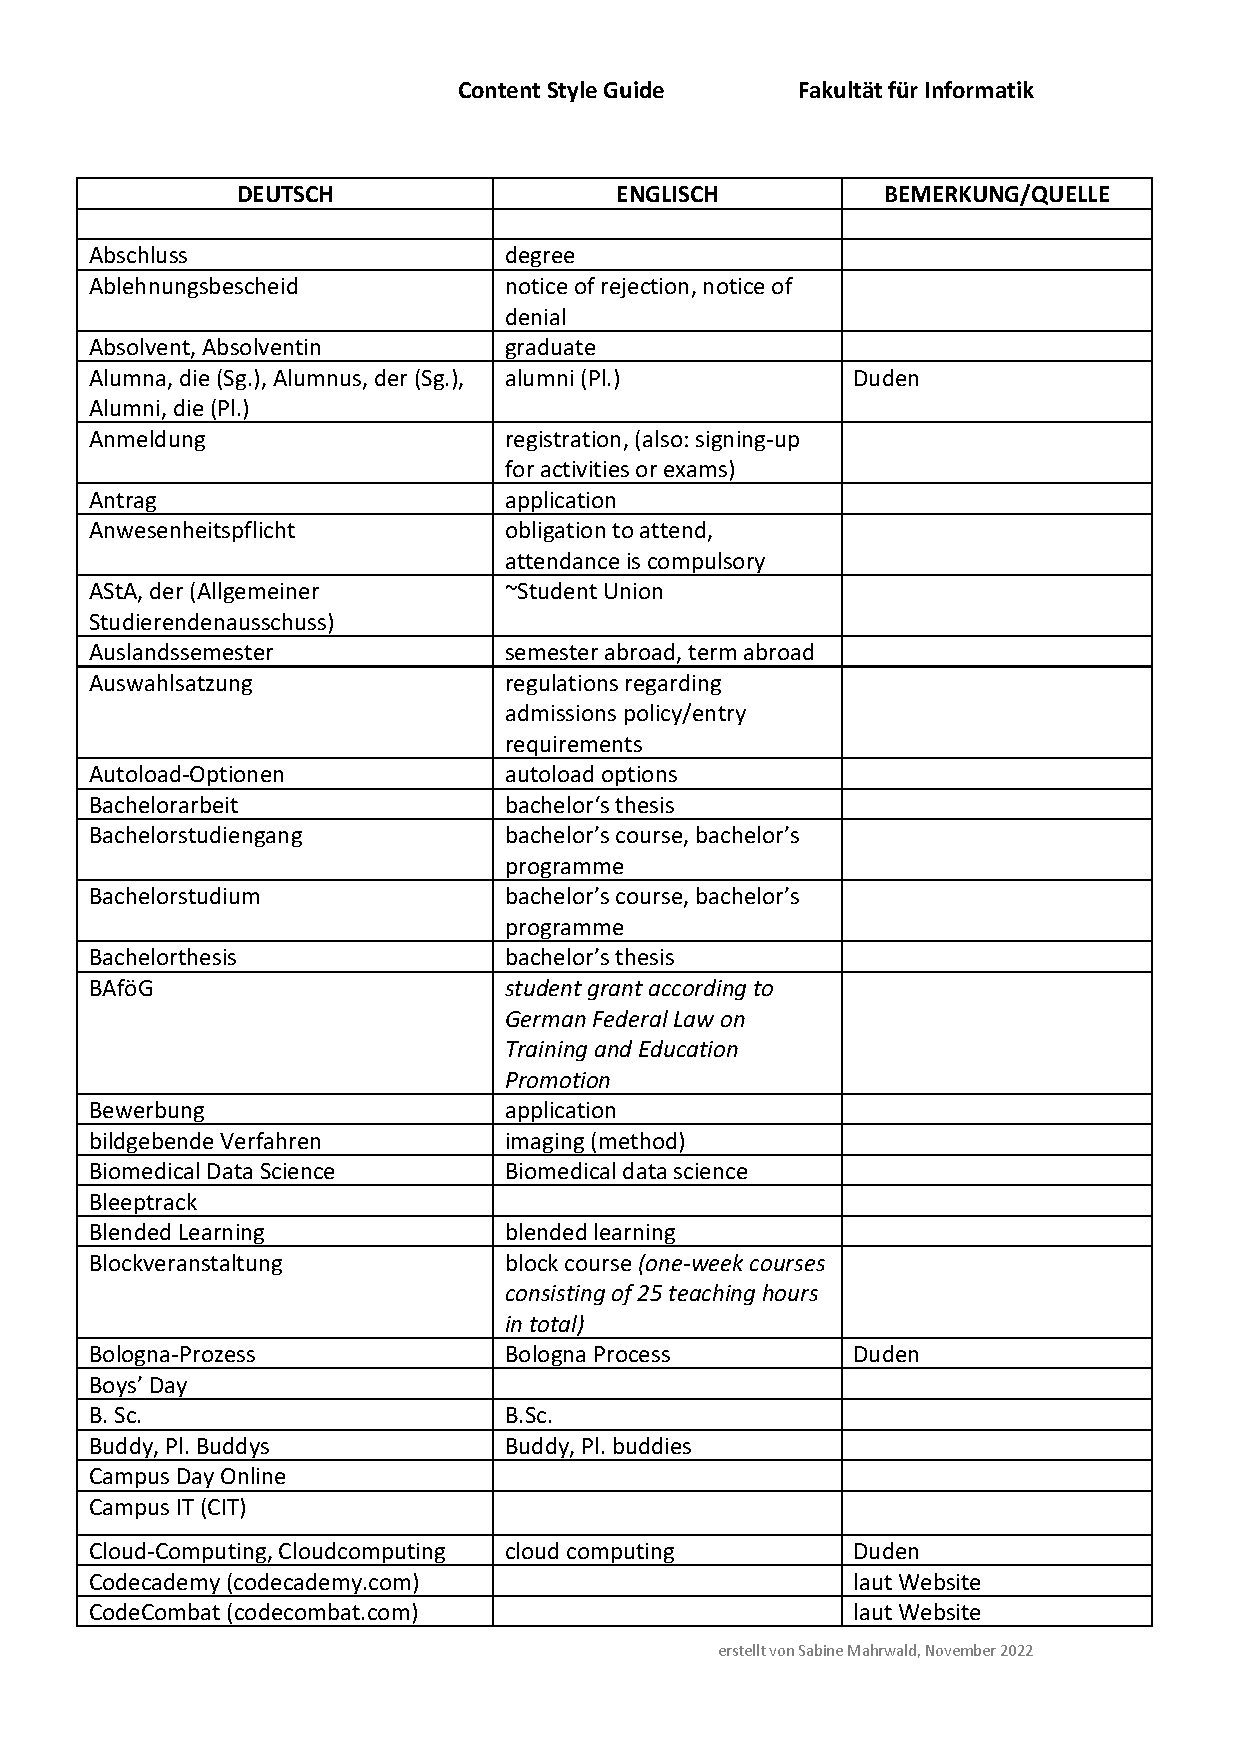
\includepdf[pages=-        % Alle Seiten des Dokumentes einbinden
           ,scale=.8      % Seiten verkleinern, damit sie zum Layout passen
           ,pagecommand={} % Layout des umgebenden Dokumentes belassen
           ]{pdfs/style_guide.pdf}



\end{document}

